\documentclass[12pt,a4paper]{article}
\usepackage[utf8]{inputenc}
\usepackage[T1]{fontenc}
\usepackage{amsmath}
\usepackage{amsfonts}
\usepackage[francais]{babel}
\usepackage{amssymb}
\usepackage{graphicx}
\usepackage[top=2.00cm]{geometry}
\usepackage{enumitem}
\usepackage{bigcenter}
\usepackage{multicol}

\usepackage{titlesec}
%modif des titres de section diminuer la taille
\renewcommand{\thesection}{\Roman{section}}
\titleformat{\section}
{\normalfont\Large\bfseries\scshape}{\thesection}{1em}{}
\titleformat{\subsection}
{\normalfont\large\bfseries}{\thesubsection}{1em}{}


\author{CHARNAY Valentin, FINOT Sylvain}
\title{Compte rendu de TP :\\ \scshape Propagation}

\begin{document}
	\maketitle
	\rule{\linewidth}{0.4pt}
	\section{Signaux électriques  dans  un  câble  coaxial.}
	\subsection{Étude à l'aide d'un générateur HF}
	On alimente un câble coaxial par un générateur HF délivrant un signal sinusoïdal, en laissant l'extrémité A'B' ouverte. On branche l'oscilloscope sur les bornes AB pour observer le comportement "anti-résonnant" du câble
	\begin{itemize}[label=$\circ$]
		\item En faisant varier la fréquence des signaux de 1MHz à 5MHz on, remarque que la déviation est maximum pour chaque multiple de 1,5MHz, on en conclue donc que la fréquence $\nu_0$=1,5MHz. Une autre façon de voir les choses, le signal fait un aller-retour en $\dfrac{1}{\nu_0}$. On peut en déduire la vitesse de propagation et donc l'indice du câble, que l'on peut relier à la permittivité diélectrique relative.
		\begin{multicols}{2}
			\begin{align*}
			v&=2l\nu_0=\dfrac{c}{n}\\
			&=2\times60\times1,5.10^6\\
			&=1,8.10^8 m/s
			\end{align*}
			\vfill
			\setlength\columnseprule{0.5pt}
			\columnbreak
			\begin{align*}
			\implies n&\equiv\sqrt{\epsilon_r}=\dfrac{c}{2l\nu_0}\\
			&=1,67\\
			\iff \epsilon_r&=n^2=2,77
			\end{align*}
		\end{multicols}
		\item On cherche à présent la plus petite déviation. Elle est obtenue en mettant une résistance de 50$\Omega$ à l'extrémité A'B'. La résistance caractéristique du câble est donc Z$_0$=50$\Omega$ 
	\end{itemize}
	\subsection{Étude à l'aide d'un générateur BF}
	On reprend le montage précédent en remplaçant le générateur HF par un générateur BF délivrant des signaux en créneaux dont la fréquence est de l'ordre de 50 kHz. On observe alors la tension entre A' et B' à l'oscilloscope (B' à la masse). On peut distinguer trois cas:
	\begin{itemize}%[label=$\circ$]
		\item la ligne est ouverte en A'B' (i.e Z=$\infty$)
		\item la ligne est en court-circuit en A'B' en court-circuit (Z$\approx 0$)
		\item la ligne est fermée sur une impédance Z
	\end{itemize}
	Occupons-nous du dernier cas qui englobe les deux premiers dans une certaine mesure :
	\begin{itemize}
		\item Z<Z$_0$ : On remarque que le signal réfléchi est soustrait au signal d'entrée.
		\item Z>Z$_0$ : Cette fois-ci, le signal réfléchi s'ajoute au signal d'entrée.
		\item  Z=Z$_0$ on supprime le signal réfléchi 
	\end{itemize}
	Dans notre cas, nous avons pu observer que le signal réfléchi était supprimé pour Z=Z$_0$=50$\Omega$
	\subsection{Étude à l'aide d'un générateur d'impulsions}
	Problème d'appareillage, impossible de synchroniser l'oscilloscope pour pouvoir faire des relevés.
	\section{Ondes acoustiques}
	\begin{itemize}
		
		\subsection{Production et nature du son}
		\item[$\circ$] Nous avons remarqué que le signal émis par le diapason est une sinusoïdal propre qui décroit en amplitude dans le temps alors que le signal émis par la table lorsqu'on la frappe frénétiquement est un signal non périodique totalement hasardeux qui s'atténue rapidement. La fréquence que nous avons mesurée pour le signal du diapason de l'ordre des 400 Hz ($\sim 442$ Hz).
		\\
		
		\item[$\circ$] En faisant varier la fréquence d'émission du haut-parleur (en multiple de 128 Hz) et en faisant varier indépendamment la distance entre le micro et le haut-parleur, nous avons remarqué que plus la fréquence est haute plus l'amplitude est faible. De plus, nous avons observé que les surfaces équipotentielles formées par le diapason sont de forme sphérique. Nous en avons déduit que le son est une superposition d'ondes sphériques.
		
		\subsection{Propagation des ondes acoustiques}
		\item[$\circ$] En faisant progressivement le vide dans l'enceinte, nous avons remarqué que l'intensité du signal devient de plus en plus faible ainsi que sa fréquence jusqu'à être nulle. Puis en rajoutant progressivement de l'air, le signal capté gagne en amplitude et en fréquence. La conclusion est alors simple et connue : le son est une onde mécanique qui nécessite de la matière pour se propager. Concrètement, le son vient d'une propagation d'une perturbation de pression locale (mélange de dépression et de surpression) dans un milieu. La perturbation se propage de proche en proche entre les molécules.
		
		\item[$\circ$] Si on relie les deux lames du diapason avec une règle en bois, nous ne captons pas de signal sonore (ou alors très succinctement). Cela vient du fait que nous atténuons la vibration des lames avec la rigidité de la règle.
		
		Cependant, en plongeant les lames dans de l'eau, le signal est bien moins atténué grâce à la viscosité de l'eau tout en gardant la même fréquence.
		
		\item[$\circ$] Pour créer un isolant acoustique, il suffit donc de recouvrir les parois intérieures du milieu de matériau ayant la capacité à amortir les chocs et à retrouver sa forme initiale. On a vu précédemment que l'éponge remplit bien cette tâche, mais d'autres matériaux ressemblant à de la mousse feraient l'affaire.
		
		\item[$\circ$] 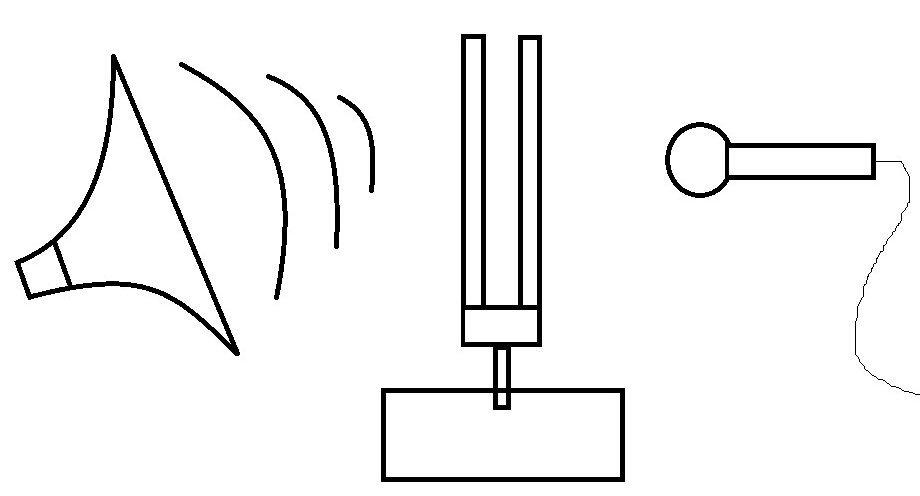
\includegraphics[scale=0.4]{schem2} \\
		
		
		En réalisant l'expérience ci-dessus, nous obtenons un signal en "double sinusoïde". En changeant progressivement la fréquence du signal du haut-parleur, nous obtenons un signal sinusoïdal classique. \\
		\begin{center}
			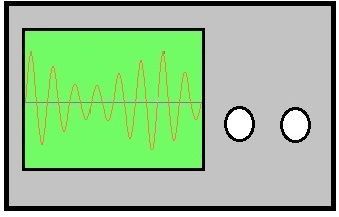
\includegraphics[scale=0.5]{schem3} $\hspace{1cm} \Rightarrow \hspace{1cm} $
			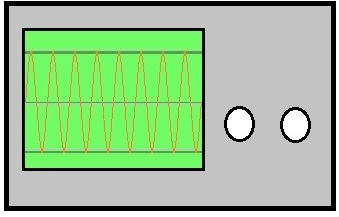
\includegraphics[scale=0.5]{schem1} 
		\end{center}
		
		La fréquence correspondant à ce signal nous donne la fréquence de résonance du diapason, lorsque l'enveloppe de notre sinusoïde est une droite. Afin de vérifier notre intuition, nous avons fait deux fois l'expérience : une avec une fréquence $\nu$ connue ($\sim 440$ Hz) et une avec une fréquence inconnue $\nu$'. Nous avons donc bien retrouvé la fréquence du diapason puis une fréquence $\nu$' d'environ 420 Hz.
		
		\item[$\circ$] Une autre méthode pour découvrir le signal du diapason consisterait à [...]
	\end{itemize}
\end{document}
